In questo capitolo ci concentreremo sulle reti di accesso a banda larga.
Il termine "banda larga" può essere ambiguo, attualmente si utilizza il termine "a banda ultra larga".
\begin{figure}[H]
	\centering
	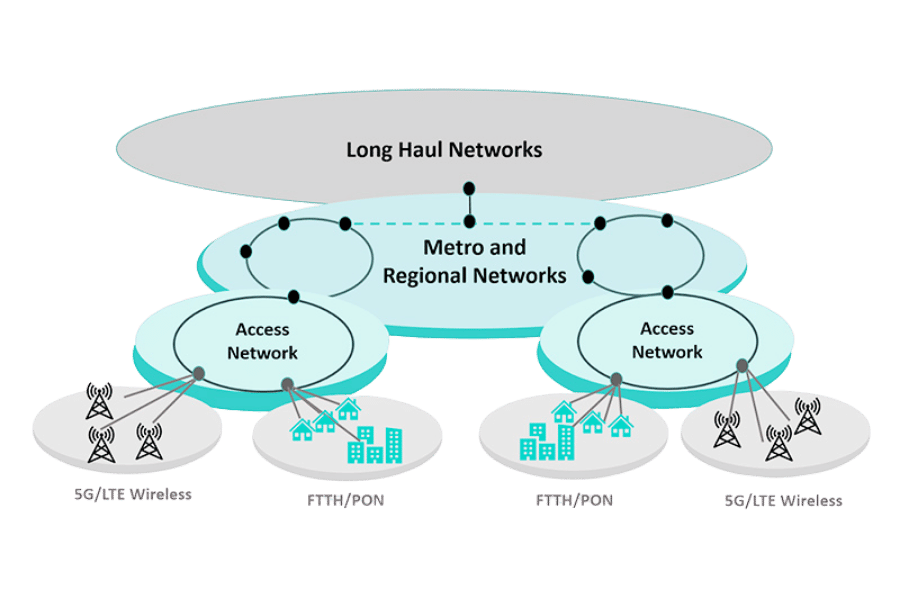
\includegraphics[width=0.8\textwidth]{pictures/2/b-62.png}
	\caption{Divisone strutturale delle reti di telecomunicazione.}
\end{figure} \noindent
Le reti di accesso a banda larga possono essere diversificate in base al medium di trasmissione utilizzato e all'architettura di rete.
\begin{itemize}
	\item \textbf{Fixed access network}: il cablaggio è effettuato fino alla casa dell'utente, ad esempio con fibra ottica o cavo coassiale. Non è prevista la mobilità dell'utente.
	\item \textbf{Fixed wireless access (FWA) network}: cablaggio in fibra fino a un point of presence (PoP) e poi connessione wireless fino alla casa dell'utente. Non è prevista la mobilità dell'utente.
	\item \textbf{Satellite access network}: cablaggio in fibra fino a una stazione radio terrestre, poi connessione satellitare fino alla casa dell'utente. Non è tipicamente prevista la mobilità dell'utente.
	\item \textbf{Mobile radio access network}: cablaggio (o collegamento radio) fino a una stazione radio base, poi comunicazione radio a un terminale mobile. È prevista la mobilità dell'utente.
\end{itemize}
\section{Fixed access network}
\begin{figure}[H]
	\centering
	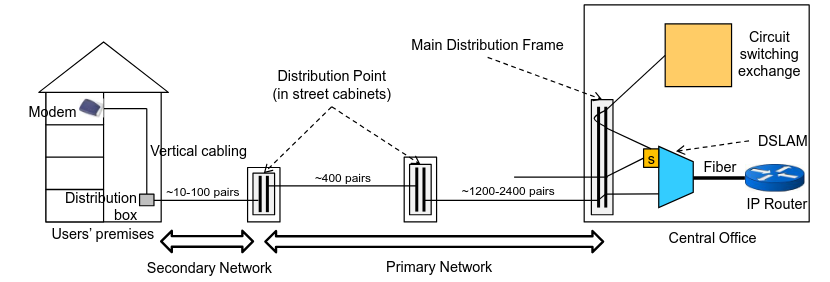
\includegraphics[width=\textwidth]{pictures/2/FAN.png}
	\caption{Infrastruttura di accesso in rame.}
\end{figure}
Analizziamo le componenti principali di una rete di accesso fissa:
\begin{itemize}
	\item \textbf{Distribution box (punto di distribuzione)}: presente nell'edificio, tipicamente in cantina.
	Permette di non collegare direttamente ogni doppino al distribution point.
	\item \textbf{Distribution point (ripartitore)}: permutatore presente in un cabinetto in strada. Effettua delle permutazioni fisiche connettendo i doppini che provengono da segmenti diversi tramite jumpers.
	Tipicamente, non vi sono più di due ripartitori tra l'utente e la centrale. Inoltre è possibile avere connessioni dirette tra centrale e utente, senza passare per un ripartitore, ma ciò è meno comune.
	\item \textbf{Main distribution Frame (permutatore)}: permutatore che permette di interfacciarsi con la rete a banda larga.
	\item \textbf{DSLAM (DSL access multiplexer)}: seleziona la porzione di banda da dedicare alla comunicazione (commutazione di pacchetto) e la comunica al router IP.
	Effettua la modulazione e demodulazione usando un array di modem, ovviamente un modem è necessario per ogni utente connesso.
\end{itemize}
È possibile utilizzare questo tipo di rete con infrastrutture originariamente progettate per la telefonia, 
ma è necessario separare le frequenze utilizzate per la telefonia da quelle utilizzate per la trasmissione dati, ad esempio con un filtro (POTS, plain old telephony splitter).
Tuttavia, queste soluzioni sono obsolete e in via di dismissione, per la telefonia si utilizzano reti VoIP (Voice over IP) che non richiedono una separazione fisica tra voce e dati.
\bigbreak\noindent
La distanza tra l'utente e la centrale dipende molto dal paese, ad esempio in Italia la distanza è molto corta, il che la rende adatta a tecnologie a banda larga.
Inoltre, la qualità dei ripartitori ha un forte impatto sulla qualità del servizio, poiché la presenza di un ripartitore può introdurre rumore e attenuazione del segnale.
\bigbreak\noindent
L'utilizzo di questa tecnologia è a basso costo, in quanto sfrutta infrastrutture già esistenti per la rete telefonica (con l'aggiunta di specifici apparati per utenti e centrali).
Vengono inoltre utilizzate per le tecnologia \textbf{xDSL} (Digital Subscriber Line).
\subsection{xDSL}
L'idea alla base delle tecnologie xDSL è quella di utilizzare la maggiorparte della banda disponibile su doppini già presenti.
Ovviamente, c'è un trade-off tra banda disponibile e distanza massima raggiungibile, poiché la banda utilizzabile è limitata dalle caratteristiche del mezzo trasmissivo.
Forme più ''aggressive'' di xDSL utilizzano bande più ampie, ma ciò comporta una riduzione della distanza massima raggiungibile.
Negli acronimi la prima lettera ''A'' sta per ''Asymmetric'', mentre la lettera ''V'' sta per ''Very high bit rate''.
\begin{table}[H]
\centering
\small
\rowcolors{2}{gray!10}{white}
\begin{tabular}{>{\raggedright\arraybackslash}p{2.2cm} >{\raggedright\arraybackslash}p{1.8cm} >{\raggedright\arraybackslash}p{1.8cm} >{\raggedright\arraybackslash}p{2.9cm} >{\raggedright\arraybackslash}p{4.8cm}}
\rowcolor{blue!20}
	\textbf{Technology} & \textbf{Standard} & \textbf{Band} & \textbf{Capacity (down/up or aggregate)} & \textbf{Maximum distance (indicative)} \\
ADSL2+ & G.992.5 & 2.2 MHz & 24/1.4 Mbit/s & A few km (approx. 3/3.5 km) \\
VDSL2 & G.993.2 17a & 17.6 MHz & 70 Mbit/s & A few hundred meters (approx. 500 m) \\
VDSL2 & G.993.2 30a & 30 MHz & 100+ Mbit/s & A few hundred meters (approx. 500 m) \\
VDSL2 & G.993.2 35b & 35 MHz & 200+ Mbit/s & A few hundred meters (approx. 500 m) \\
G.fast & G.9700/9701 & 106/212 MHz & 700 Mbit/s & A few tens of meters (less than 100 m) \\
\end{tabular}
\caption{Confronto tra principali tecnologie xDSL.}
\end{table}
\begin{figure}[H]
\centering
\resizebox{0.95\textwidth}{!}{%
\begin{tikzpicture}[>=Stealth, font=\scriptsize]

% ===== ADSL2+ =====
\draw[->, thick] (0.5,5.6) -- (10.0,5.6);
\node[right] at (9.9,5.85) {ADSL2+};

\draw[fill=gray!35, thick, rounded corners=5pt] (0.5,5.6) rectangle (1.55,6.35);
\node at (1.025,5.98) {\textbf{POTS}};

\draw[fill=yellow!90, thick, rounded corners=5pt] (1.95,5.6) rectangle (3.6,6.35);
\node at (2.775,5.98) {\textbf{UP}};

\draw[fill=green!70!black!20, thick, rounded corners=5pt] (3.6,5.6) rectangle (6.55,6.35);
\node at (5.075,5.98) {\textbf{DOWN}};

\node[anchor=north east] at (1.9,5.28) {4kHz};
\node[anchor=north west] at (1.8,5.28) {26kHz};
\node[anchor=north] at (3.6,5.28) {138kHz};
\node[anchor=north] at (6.55,5.3) {2.3 MHz};

% ===== VDSL2 35b =====
\draw[->, thick] (0.5,3.75) -- (10.0,3.75);
\node[right] at (9.8,4.02) {VDSL2 (G.993.2 35b)};

\draw[fill=gray!35, thick, rounded corners=5pt] (0.5,3.75) rectangle (1.5,4.5);
\node at (1.0,4.12) {\textbf{POTS}};

\draw[fill=yellow!90, thick, rounded corners=5pt] (1.9,3.75) rectangle (3.6,4.5);
\node at (2.75,4.12) {\textbf{UP}};

\draw[shade, left color=yellow!70, right color=green!60, draw=black, thick, rounded corners=5pt]
	(3.6,3.75) rectangle (8.1,4.5);
\node at (5.85,4.12) {\textbf{UP/DOWN FDD}};

\node[anchor=north east] at (1.9,3.43) {4kHz};
\node[anchor=north west] at (1.8,3.43) {26kHz};
\node[anchor=north] at (3.6,3.43) {138kHz};
\node[anchor=north] at (8.1,3.45) {35 MHz};

% ===== G.fast =====
\draw[->, thick] (0.5,1.9) -- (10.0,1.9);
\node[right] at (9.8,2.16) {G.fast};

\draw[fill=gray!35, thick, rounded corners=5pt] (2.7,1.9) rectangle (4.9,2.65);
\draw[fill=gray!35, thick, rounded corners=5pt] (4.55,1.9) rectangle (6.5,2.65);

\draw[shade, left color=yellow!70, right color=green!60, draw=black, thick, rounded corners=5pt]
	(6.1,1.9) rectangle (9.5,2.65);
\node at (7.85,2.27) {\textbf{TDD}};

\node[anchor=north] at (2.7,1.58) {138kHz};
\node[anchor=north] at (4.55,1.58) {2.3 MHz};
\node[anchor=north] at (6.1,1.58) {35 MHz};
\node[anchor=north] at (9.5,1.58) {212 MHz};

\end{tikzpicture}%
}
\caption{Allocazione semplificata in frequenza per ADSL2+, VDSL2 35b e G.fast.}
\end{figure}\noindent
In VDSL2, è possibile utilizzare la tecnica FDD (Frequency Division Duplexing) per separare le frequenze dedicate alla trasmissione in upstream da quelle dedicate alla trasmissione in downstream.
In G.fast, invece, si utilizza la tecnica TDD (Time Division Duplexing), che consente di utilizzare la stessa banda per entrambe le direzioni di comunicazione, alternando nel tempo le trasmissioni in upstream e downstream.
\subsection{Vectoring}
Tecnologia ideata per mitigare il fenomeno del crosstalk, ovvero l'interferenza tra coppie di cavi adiacenti.
Il crosstalk è la maggiore fonte di rumore. Inoltre il vectoring migliora le performance.
I segnali ricevuti $r_1$ e $r_2$ su due coppie adiacenti vengono disturbati dai reciproci crosstalk $k_1$ e $k_2$.
\begin{align*}
	r_1 &= s_1 + k_1 s_2 \\
	r_2 &= s_2 + k_2 s_1
\end{align*}
In forma matriciale, possiamo scrivere:
\begin{align*}
	\vec{r} &= T \vec{s}\\
	T&=\begin{bmatrix}1 & k_1 \\ k_2 & 1 \end{bmatrix}
\end{align*}
Trasmettendo il segnale $\vec{s}\phantom{.} ^*= T^{-1} \vec{s}$ (preconding) il segnale desiderato $\vec{s}$ viene ricevuto senza interferenze:
\begin{align*}
	\vec{r} &= T \vec{s}\phantom{.} ^* = T T^{-1} \vec{s} = \vec{s}
\end{align*}
Queste operazioni vengono effettuate dal DSLAM in direzione di downstream.
Nella direzione di upstream, invece, il crosstalk viene cancellato a priori dal DSLAM:
\begin{align*}
	\vec{r} &= T^{-1} (T\vec{s})=\vec{s}
\end{align*}
Il vectoring presenta due limitazioni principali:
\begin{itemize}
	\item $T$ deve essere calcolata dinamicamente su un grande numero di doppini, poiché le condizioni di crosstalk possono variare nel tempo. Inoltre questa operazione è computazionalmente costosa.
	\item Benefici molto limitati se diversi ISP (internet service providers) coesistono nella gestione della rete.
\end{itemize}
\section{Reti fibra misto rame}
Come già accennato, c'è un trade-off tra banda disponibile e distanza massima raggiungibile, poiché la banda utilizzabile è limitata dalle caratteristiche del mezzo trasmissivo.
I cavi in fibra ottica offrono una banda molto più ampia rispetto ai cavi in rame, ma sono più costosi da installare e mantenere.
Per questo motivo, una soluzione comune è quella di utilizzare una rete fibra misto rame (Fiber to the X, FTTX), i
in cui la fibra ottica viene utilizzata fino a un certo punto della rete, e poi si utilizza il rame per raggiungere l'utente finale.
Le varie soluzioni FTTX si differenziano in base a dove termina la fibra ottica.
\subsection{Fiber to the exchange (FTTE)}
In questa soluzione, la fibra ottica termina presso la centrale telefonica (exchange), e il rame viene utilizzato per collegare la centrale agli utenti finali.
È esattamente la soluzione vista nella sezione precedente, in cui si utilizzano tecnologie xDSL per la trasmissione dati sul rame.
\begin{figure}[H]
	\centering
	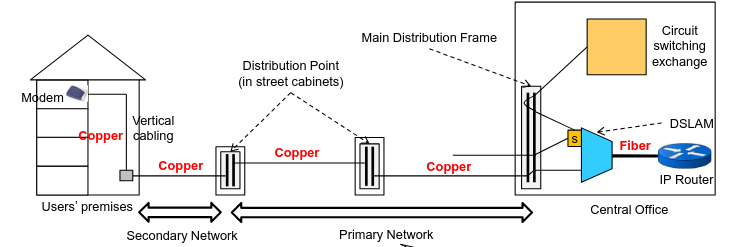
\includegraphics[width=0.8\textwidth]{pictures/2/FTTE.png}
	\caption{Architettura di rete Fiber to the Exchange (FTTE).}
\end{figure}\noindent
Vengono utilizzati doppini sia nella primary che nella secondary network.
\subsection{Fiber to the cabinet (FTTC)}
In questa soluzione, la fibra ottica termina presso un cabinetto in strada (cabinet), e il rame viene utilizzato per collegare il cabinet agli utenti finali.
Il cabinet è un dispositivo attivo, che necessita di alimentazione elettrica, e contiene un DSLAM che effettua la modulazione e demodulazione dei segnali.
\begin{figure}[H]
	\centering
	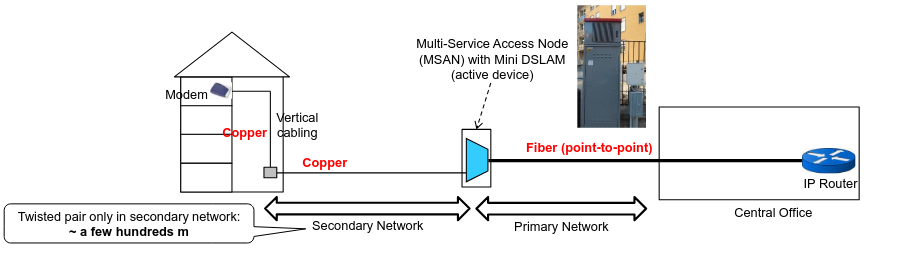
\includegraphics[width=0.9\textwidth]{pictures/2/FTTC.png}
	\caption{Architettura di rete Fiber to the Cabinet (FTTC).}
\end{figure}\noindent
I doppini vengono utilizzati solo nella secondary network, mentre nella primary network viene utilizzata la fibra ottica.
\subsection{Fiber to the building (FTTB)}
In questa soluzione, la fibra raggiunge l'edificio degli utenti (tipicamente in cantina), dove viene installato un mini DSLAM.
I doppini degli utenti forniscono alimentazione al mini DSLAM (reverse power feeding), che effettua la modulazione e demodulazione dei segnali.
\begin{figure}[H]
	\centering
	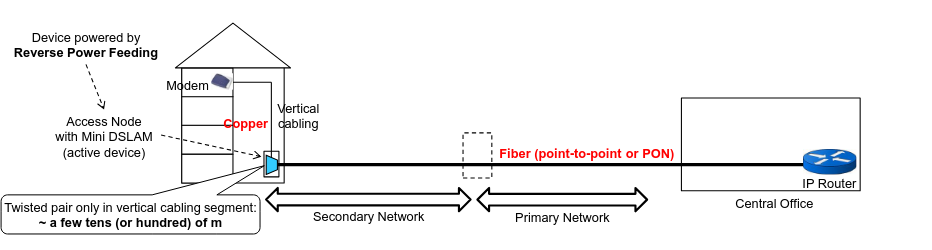
\includegraphics[width=0.9\textwidth]{pictures/2/FTTB.png}
	\caption{Architettura di rete Fiber to the Building (FTTB).}
\end{figure}\noindent
Soluzione non molto comune, poiché è necessario installare un mini DSLAM per ogni edificio, ma offre prestazioni migliori rispetto a FTTC. Inoltre risulta poco conveniente
per i fornitori di servizi, poiché è necessario installare un mini DSLAM per ogni edificio, e ciò comporta costi elevati.
\subsection{Fiber to the home (FTTH)}
In questa soluzione, la fibra ottica raggiunge direttamente la casa dell'utente, eliminando l'utilizzo del rame.
Ci sono due principali architetture di rete utilizzate in FTTH: PON (Passive Optical Network) e Point-to-Point (P2P).
\begin{figure}[H]
	\centering
	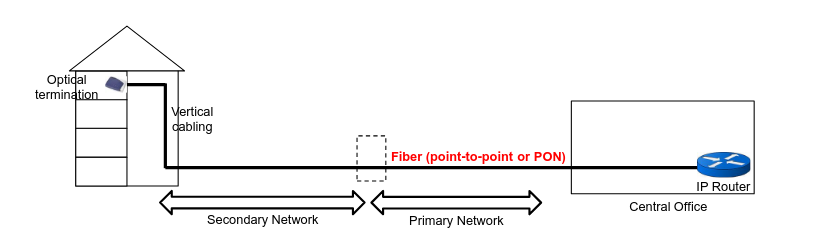
\includegraphics[width=0.9\textwidth]{pictures/2/FTTH_P2P.png}
	\caption{Architettura di rete Fiber to the Home (FTTH) con Point-to-Point (P2P).}
\end{figure}\noindent
Nell'architettura P2P, ogni utente ha una connessione dedicata in fibra ottica fino alla centrale, offrendo prestazioni elevate ma a costi più elevati dato l'elevata quantità di cavi necessaria.\
Il multiplexing/demultiplexing viene effettuato al MPoP (Metropolitan Point of Presence). Viene adottata principalmente come soluzione business (anche se spesso in realtà per questi utilizzatori si utilizza comunque la PON).
\begin{figure}[H]
	\centering
	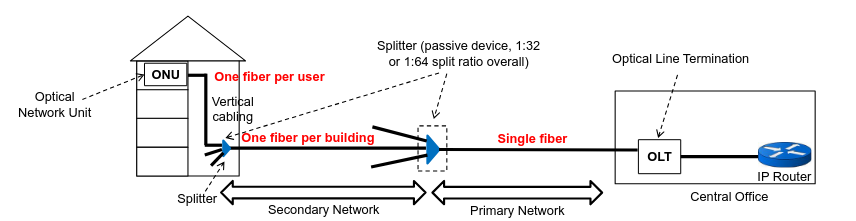
\includegraphics[width=0.9\textwidth]{pictures/2/FTTH_PON.png}
	\caption{Architettura di rete Fiber to the Home (FTTH) con Passive Optical Network (PON).}
\end{figure}\noindent
Nelle reti PON viene creata una rete ad albero, in cui la fibra ottica viene condivisa tra più utenti tramite un dispositivo di splitting passivo (splitter), che divide il segnale ottico in più segnali per raggiungere gli utenti finali.
Richiede meno cavi rispetto alla soluzione P2P, ma offre prestazioni inferiori a causa della condivisione della banda tra gli utenti.
Viene adottata principalmente come soluzione residenziale.
In downstream la trasmissione avviene in broadcast, ogni utente filtra il proprio traffico, mentre in upstream si usa un TDMA (Time Division Multiple Access) gestito dal OLT (Optical Line Terminal) che assegna slot temporali agli utenti per evitare collisioni.
Questa tecnologia può essere adottata anche per architetture del tipo FTTB, in modo da ridurre significativamente i costi (viene comunque fatto reverse power feeding).
\section{Fixed wireless access}
Spesso viene chiamato anche fiber to the tower (FTTT), poiché la fibra ottica raggiunge una stazione radio base (tower) da cui poi si effettua
la connessione wireless fino alla casa dell'utente.
È una soluzione più economica e flessibile delle reti di accesso fisse. Tipicamente viene adottata in montagna, aree rurali o zone dove non sarebbe conveniente installare una rete di accesso fissa.
Risulta un'ottima soluzione per ridurre il divario digitale.
\begin{figure}[H]
	\centering
	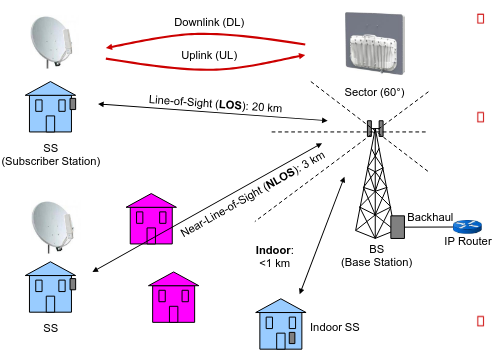
\includegraphics[width=0.7\textwidth]{pictures/2/FWA.png}
	\caption{Architettura di rete Fixed Wireless Access (FWA).}
	\label{fig:FWA}
\end{figure}\noindent
La stazione radio base è collegata alla rete tramite fibra ottica, e comunica con i terminali degli utenti tramite onde radio.
Facendo riferimento alla figura \ref{fig:FWA} possiamo identificare i vari tipi di comunicazioni wireless:
\begin{itemize}
	\item \textbf{LOS}: Line of Sight, comunicazione diretta tra stazione radio base e terminale dell'utente, senza ostacoli (situazione outdoor).
	\item \textbf{NLOS}: Non Line of Sight, comunicazione indiretta tra stazione radio base e terminale dell'utente, con ostacoli (situazione outdoor).
	\item \textbf{Indoor}: La base station e la subscriber station sono molto vicine, e la comunicazione avviene all'interno di un edificio (situazione indoor).
	\item \textbf{Backhaul}: Collegamento in fibra ad alta velocità.
\end{itemize}
La trasmissione e ricezione avvengono per mezzo di potenti antenne direzionali per quanto riguarda la subscriber station in LOS o NLOS con la base station.
Per la situazione indoor, invece, si utilizzano antenne omnidirezionali, mentre la base station utilizza antenne settoriali con MIMO.
\section{Reti satellitari}
\begin{figure}[H]
	\centering
	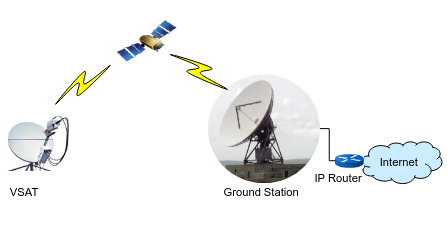
\includegraphics[width=0.5\textwidth]{pictures/2/SAT.png}
	\caption{Architettura di rete satellitare.}
\end{figure}\noindent
Offrono una copertura globale, come FWA sono una soluzione ideale per aree rurali o remote dove non è conveniente installare una rete di accesso fissa.
Per costruire una rete satellitare sono necessari:
\begin{itemize}
	\item \textbf{VSAT}: very small aperture terminal, terminale dell'utente (antenna parabolica) che comunica con il satellite.
	\item \textbf{Stazione di terra}: stazione terrestre che comunica con il satellite e si collega alla rete tramite fibra ottica. Una parabola con grande apertura.
\end{itemize}
La comunicazione in questa maniera introduce una latenza non trascurabile, dato che la comunicazione avviene tra stazione di terra $\rightarrow$ satellite $\rightarrow$ satellite $\rightarrow$ stazione di terra $\rightarrow$ VSAT, e viceversa.
Inoltre, un aspetto fondamentale è la distanza dei satelliti dal pianeta, dato che satelliti troppo distanti non possono essere utilizzati per applicazioni real-time.
\begin{itemize}
	\item \textbf{LEO (Low Earth Orbit)}: orbita a bassa quota, con satelliti a circa 500-2000 km di altitudine. Offrono latenza più bassa (circa 20-40 ms). 
	I satelliti si muovono rapidamente rispetto la terra, di conseguenza la gestione della rete è molto complessa.
	\item \textbf{MEO (Medium Earth Orbit)}: orbita a media quota, con satelliti a circa 2000-35.000 km di altitudine. Non vengono usati per accesso a internet.
	\item \textbf{GEO (Geostationary)}: orbita geostazionaria, con satelliti a circa 35.786 km di altitudine. Offrono latenza elevata (circa 500 ms) ma richiedono solo pochi satelliti per garantire la copertura globale.
	Il piano orbitale coincide con l'equatore, quindi la velocità di rotazione del satellite è uguale a quella della terra, dunque la posizione rispetto all'orizzonte è fissa.
	Questo permette di utilizzare semplicemente delle antenne fisse in una direzione specifica. Tuttavia, non sono in grado di servire i poli terrestri.
\end{itemize}

\subsection{Reti satellitari con satelliti GEO}
Nel caso GEO, le bande più usate per accesso a Internet e servizi broadcast sono:
\begin{itemize}
	\item \textbf{Banda C}: circa 4--6 GHz.
	\item \textbf{Banda Ku}: circa 11--14 GHz.
	\item \textbf{Banda Ka}: circa 20--30 GHz.
\end{itemize}
\noindent
La copertura è molto ampia: un satellite GEO può arrivare a coprire fino a circa \(1/3\) della superficie terrestre visibile.
\noindent
Si distinguono due modalità principali di copertura:
\begin{itemize}
	\item \textbf{Single beam}: l'area è servita da un unico fascio alla stessa frequenza. È una soluzione semplice, ma con banda disponibile limitata.
	\item \textbf{Multibeam (spot beam)}: il satellite genera più fasci su aree diverse. In questo modo è possibile riusare le frequenze tra spot beam differenti e aumentare la capacità totale.
	\begin{itemize}
		\item Valori tipici: decine di spot beam (ad esempio ~80) e capacità aggregata dell'ordine di centinaia di Mbit/s (ad esempio ~900 Mbit/s).
	\end{itemize}
\end{itemize}

Per la condivisione delle risorse radio:
\begin{itemize}
	\item \textbf{Downstream}: multiplazione TDM.
	\item \textbf{Upstream}: accesso multiplo TDMA oppure CDMA.
\end{itemize}

\begin{figure}[H]
\centering
\begin{tikzpicture}[>=Stealth, font=\footnotesize]
% Single beam (sinistra)
\draw[fill=blue!60, thick] (1.8,3.8) ellipse (0.28 and 0.12);
\draw[thick] (1.6,3.7) -- (2.0,3.9);
\draw[thick] (1.58,3.9) -- (2.02,3.7);

\draw[thick] (1.8,3.75) -- (1.0,2.3);
\draw[thick] (1.8,3.75) -- (2.6,2.3);
\draw[fill=yellow!30, thick] (1.8,2.2) ellipse (1.0 and 0.35);
\node at (1.8,1.6) {Single beam};

% Multibeam (destra)
\draw[fill=blue!60, thick] (5.8,3.4) ellipse (0.28 and 0.12);
\draw[thick] (5.6,3.3) -- (6.0,3.5);
\draw[thick] (5.58,3.5) -- (6.02,3.3);

\draw[thick] (5.8,3.35) -- (4.9,2.0);
\draw[thick] (5.8,3.35) -- (5.8,2.0);
\draw[thick] (5.8,3.35) -- (6.7,2.0);

\draw[fill=yellow!35, thick] (4.9,1.9) ellipse (0.35 and 0.18);
\draw[fill=green!55, thick] (5.8,1.72) ellipse (0.4 and 0.2);
\draw[fill=orange!85, thick] (6.7,1.9) ellipse (0.35 and 0.18);
\node at (5.8,1.2) {Spot beam / multibeam};
\end{tikzpicture}
\caption{Copertura GEO: confronto tra single beam e multibeam (spot beam).}
\end{figure}

\subsection{Reti satellitari con satelliti LEO}
Le reti LEO rappresentano la soluzione satellitare più recente e dinamica per accesso a Internet a bassa latenza.

\begin{itemize}
	\item \textbf{Operatori principali}: Starlink ed Eutelsat/OneWeb.
	\item \textbf{Bande radio impiegate}: soprattutto \textbf{Ku} e \textbf{Ka}.
	\item \textbf{Dimensioni satelliti}: satelliti relativamente piccoli e leggeri (ordine di ~1 m, ~100--300 kg).
	\item \textbf{Capacità attese}: in molti scenari, ordini di grandezza pari a decine o centinaia di Mbit/s per utente (ad esempio 50--150 Mbit/s).
\end{itemize}
\noindent
Per funzionare su scala globale, le reti LEO richiedono molte \textbf{stazioni di terra} distribuite nel mondo:
\begin{itemize}
	\item OneWeb: circa 60 portali satellitari (SNP).
	\item Starlink: rete molto più estesa, con migliaia di gateway e stazioni (in forte evoluzione).
\end{itemize}

\subsubsection*{Costellazioni LEO}
La continuità del servizio è ottenuta con costellazioni composte da centinaia/migliaia di satelliti su orbite diverse (incluse orbite polari).

\begin{itemize}
	\item \textbf{Starlink}: piano molto ambizioso (fino a decine di migliaia di satelliti nel lungo periodo), con migliaia già operativi.
	\item \textbf{OneWeb}: costellazione più contenuta (ordine di alcune centinaia di satelliti), completata nella configurazione iniziale.
\end{itemize}
\noindent
Un riferimento utile per visualizzare costellazioni e orbite in tempo reale è:
\begin{center}
\url{https://satellitemap.space/}
\end{center}

\subsubsection*{Principio di funzionamento (semplificato)}
\begin{enumerate}
	\item Il terminale utente identifica i satelliti LEO visibili.
	\item Si collega al satellite più adatto (tipicamente il più vicino/affidabile in quell'istante).
	\item Quando il satellite esce dal campo visivo, avviene un \textbf{handover} verso un altro satellite visibile.
\end{enumerate}
\noindent
Nel prossimo sviluppo delle reti LEO, il \textbf{satellite routing} (instradamento diretto tra satelliti) è rilevante perché:
\begin{itemize}
	\item riduce la latenza su alcune tratte lunghe;
	\item riduce il numero di stazioni di terra necessarie in certe aree.
\end{itemize}

